\documentclass[tikz,border=15pt]{standalone}
\usepackage{tikz}
\usetikzlibrary{shapes.geometric, arrows.meta, positioning}

\tikzset{
    register/.style={
        rectangle, draw=black, thick,
        minimum width=1.4cm, minimum height=0.95cm,
        fill=white, font=\small\ttfamily
    },
    wire/.style={draw=black, thick, -Stealth},
    bus/.style={draw=black, line width=1.8pt, -Stealth},
    controlwire/.style={draw=black!60, dashed, -Stealth},
    buswidth/.style={font=\scriptsize, fill=white, inner sep=2pt},
    logic/.style={
        rectangle, draw=black, thick, rounded corners=3pt,
        minimum width=1.1cm, minimum height=0.95cm,
        fill=gray!10, font=\small
    }
}

\begin{document}
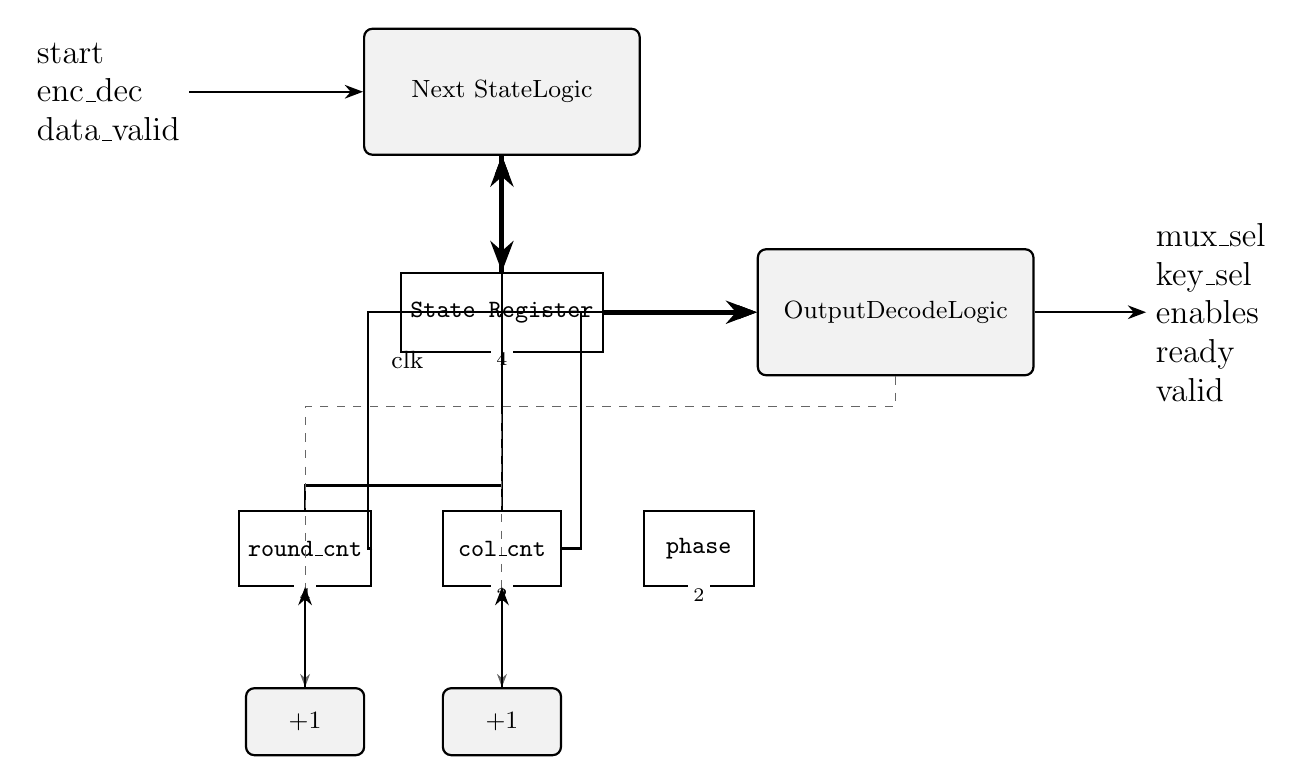
\begin{tikzpicture}

% State register (center)
\node[register, minimum width=2.5cm, minimum height=1cm] (state) at (4,4) {State Register};
\node[buswidth] at (4,3.4) {4};
\node[font=\small] at (2.8,3.4) {clk};

% Next state logic (above)
\node[logic, minimum width=3.5cm, minimum height=1.6cm] (nsl) at (4,6.8) {Next State\\Logic};

% Output/decode logic (right)
\node[logic, minimum width=3.5cm, minimum height=1.6cm] (out) at (9,4) {Output\\Decode\\Logic};

% Counters (below state)
\node[register, minimum width=1.5cm, minimum height=0.95cm] (rc) at (1.5,1) {round\_cnt};
\node[buswidth] at (1.5,0.4) {4};

\node[register, minimum width=1.5cm, minimum height=0.95cm] (cc) at (4,1) {col\_cnt};
\node[buswidth] at (4,0.4) {2};

\node[register, minimum width=1.4cm, minimum height=0.95cm] (ph) at (6.5,1) {phase};
\node[buswidth] at (6.5,0.4) {2};

% Increment logic
\node[logic, minimum width=1.5cm, minimum height=0.85cm] (inc1) at (1.5,-1.2) {+1};
\node[logic, minimum width=1.5cm, minimum height=0.85cm] (inc2) at (4,-1.2) {+1};

% External inputs (left)
\node[font=\large, align=left, text centered] (inputs) at (-1,6.8) {start\\enc\_dec\\data\_valid};

% Control outputs (right)
\node[font=\large, align=left, text centered] (outputs) at (13,4) {mux\_sel\\key\_sel\\enables\\ready\\valid};

% Dataflow connections
\draw[bus] (state) -- (nsl);
\draw[bus] (nsl) -- (state);
\draw[bus] (state) -- (out);

\draw[wire] (rc) -- ++(0,0.8) -| (nsl);
\draw[wire] (cc) -- ++(0,1) -| (nsl);
\draw[wire] (rc) -- ++(0.8,0) |- (out);
\draw[wire] (cc) -- ++(1,0) |- (out);

% Counter control
\draw[controlwire] (out) -- ++(0,-1.2) -| (inc1.north);
\draw[controlwire] (out) -- ++(0,-1.2) -| (inc2.north);
\draw[wire] (inc1) -- (rc);
\draw[wire] (inc2) -- (cc);

% External connections
\draw[wire] (inputs) -- (nsl);
\draw[wire] (out) -- (outputs);

\end{tikzpicture}
\end{document}
